% see A1.1a
\chapter{Informieren} \label{ch:inform}

\section{Projektmanagement}

Das Projekt wird nach der Projektmanagementmethode \emph{IPERKA} abgewickelt. Diese Methode eignet sich besonders gut
für ein derartiges Projekt, da das Projekt in einer einzigen Iteration innerhalb von 10 Tagen wasserfallartig realisiert werden soll.

\subsection{Arbeitspakete}

Der Auftrag kann in folgende Arbeitspakete aufgeteilt und nach den sechs Phasen der gewählten Projektmanagementmethode gegliedert werden:

\begin{itemize}
    \item \textbf{I}nformieren: Was soll getan werden? (\hyperref[ch:inform]{Kapitel \ref*{ch:inform}})
          \begin{description}
              \item[AP1: Anforderungen analysieren] Der Auftrag wird analysiert und daraus einzelne Arbeitspakete abgeleitet.
              \item[AP2: Einordnung des Systems in das Gesamtsystem] Das System, dessen Schnittstellen und die Akteure werden analysiert.
          \end{description}
    \item \textbf{P}lanen: Welche Lösungswege gibt es und wie kann man vorgehen? (\hyperref[ch:plan]{Kapitel \ref*{ch:plan}})
          \begin{description}
              \item[AP3: Anwendungsfälle definieren] Funktionalitäten der Software werden ausgehend von den Benutzerrollen dargestellt.
              \item[AP4: Datenmodelle erstellen] Aufgrund der Auftragsbeschreibung werden Entitäten definiert und deren Verhältnis zueinander aufgezeigt.
              \item[AP5: Zustandsdiagramm erstellen] Die Zustände (States) einer Assessment-Session und die dazwischenliegenden Übergänge werden dargestellt.
              \item[AP6: Testkonzept] Wie und was wird getestet? Testfälle werden definiert und verschiedenen Arten von Tests aufgezeigt.
              \item[AP7: UI-Design] Konzepte der drei Benutzer-Flows und grobe UI-Designs einzelner Seiten erstellen.
          \end{description}
    \item \textbf{E}ntscheiden: Für welches Vorgehen entscheiden man sich? (\hyperref[ch:decide]{Kapitel \ref*{ch:decide}})
          \begin{description}
              \item[AP8: Variantenvergleich und Nutzwertanalyse] Aufgrund von Objektiven Analysen werden Entscheidungen bezogen auf die Planungsphase getroffen.
          \end{description}
    \item \textbf{R}ealisieren: Die eigentliche Umsetzung des Projektes (\hyperref[ch:implement]{Kapitel \ref*{ch:implement}})
          \begin{description}
              \item[AP9: Datenmodell] Umsetzung des Datenmodells, welches in der Planungsphase erstellt wurde.
              \item[AP10: Benutzerrollen] Authentifizierung und Autorisierung verschiedener Benutzerrollen ermöglichen.
              \item[AP11: Benutzer-Flows] Realisation der drei verschiedenen Benutzer-Flows.
              \item[AP12: E-Mails] E-Mail Benachrichtigungen und Einladungen für die Bewerber umsetzen.
              \item[AP13: UI-Design] Umsetzung und Verbesserung des UI/UX basierend auf den Mockups, die in der Planungsphase erstellt wurden.
          \end{description}
    \item \textbf{K}ontrollieren: Wurde das Projekt korrekt umgesetzt? (\hyperref[ch:check]{Kapitel \ref*{ch:check}})
          \begin{description}
              \item[AP14: Anforderungen überprüfen] Die Anforderungen werden nochmals analysiert - wurde alles beachtet?
              \item[AP15: Testing] Sowohl manuelle als auch automatisierte Tests werden durchgeführt und ein jeweiliger Testbericht wird erfasst.
          \end{description}
    \item \textbf{A}uswerten: Was ist gelungen, was nicht? (\hyperref[ch:evaluate]{Kapitel \ref*{ch:evaluate}})
          \begin{description}
              \item[AP16: Reflektieren] Das Endergebnis der PA wird bezogen auf die Aufgabenstellung evaluiert und der Arbeitsprozess reflektiert.
          \end{description}
\end{itemize}

\newpage

\section{Systemaufbau}

Im folgenden Abschnitt wird die Einordnung des Systems in das Gesamtsystem gezeigt, sowie die vorhandenen Schnittstellen und Akteure beschrieben.

\subsection{Gesamtsystem}

Die Abbildung \ref{fig:deployment} zeigt die Zusammenhänge der einzelnen Systeme, die in dieser PA zum Einsatz kommen.
Der Kern des Gesamtsystems ist hierbei die \emph{Ruby on Rails} Applikation, die auf einem Heroku Cloud-Server gehostet werden soll.

Es wurden nur die notwendigsten Komponenten der einzelnen Nodes aufgezeigt, welche über die jeweiligen Schnittstellen direkt mit den anderen Systemen interagieren.

\begin{figure}[H]
    \centering
    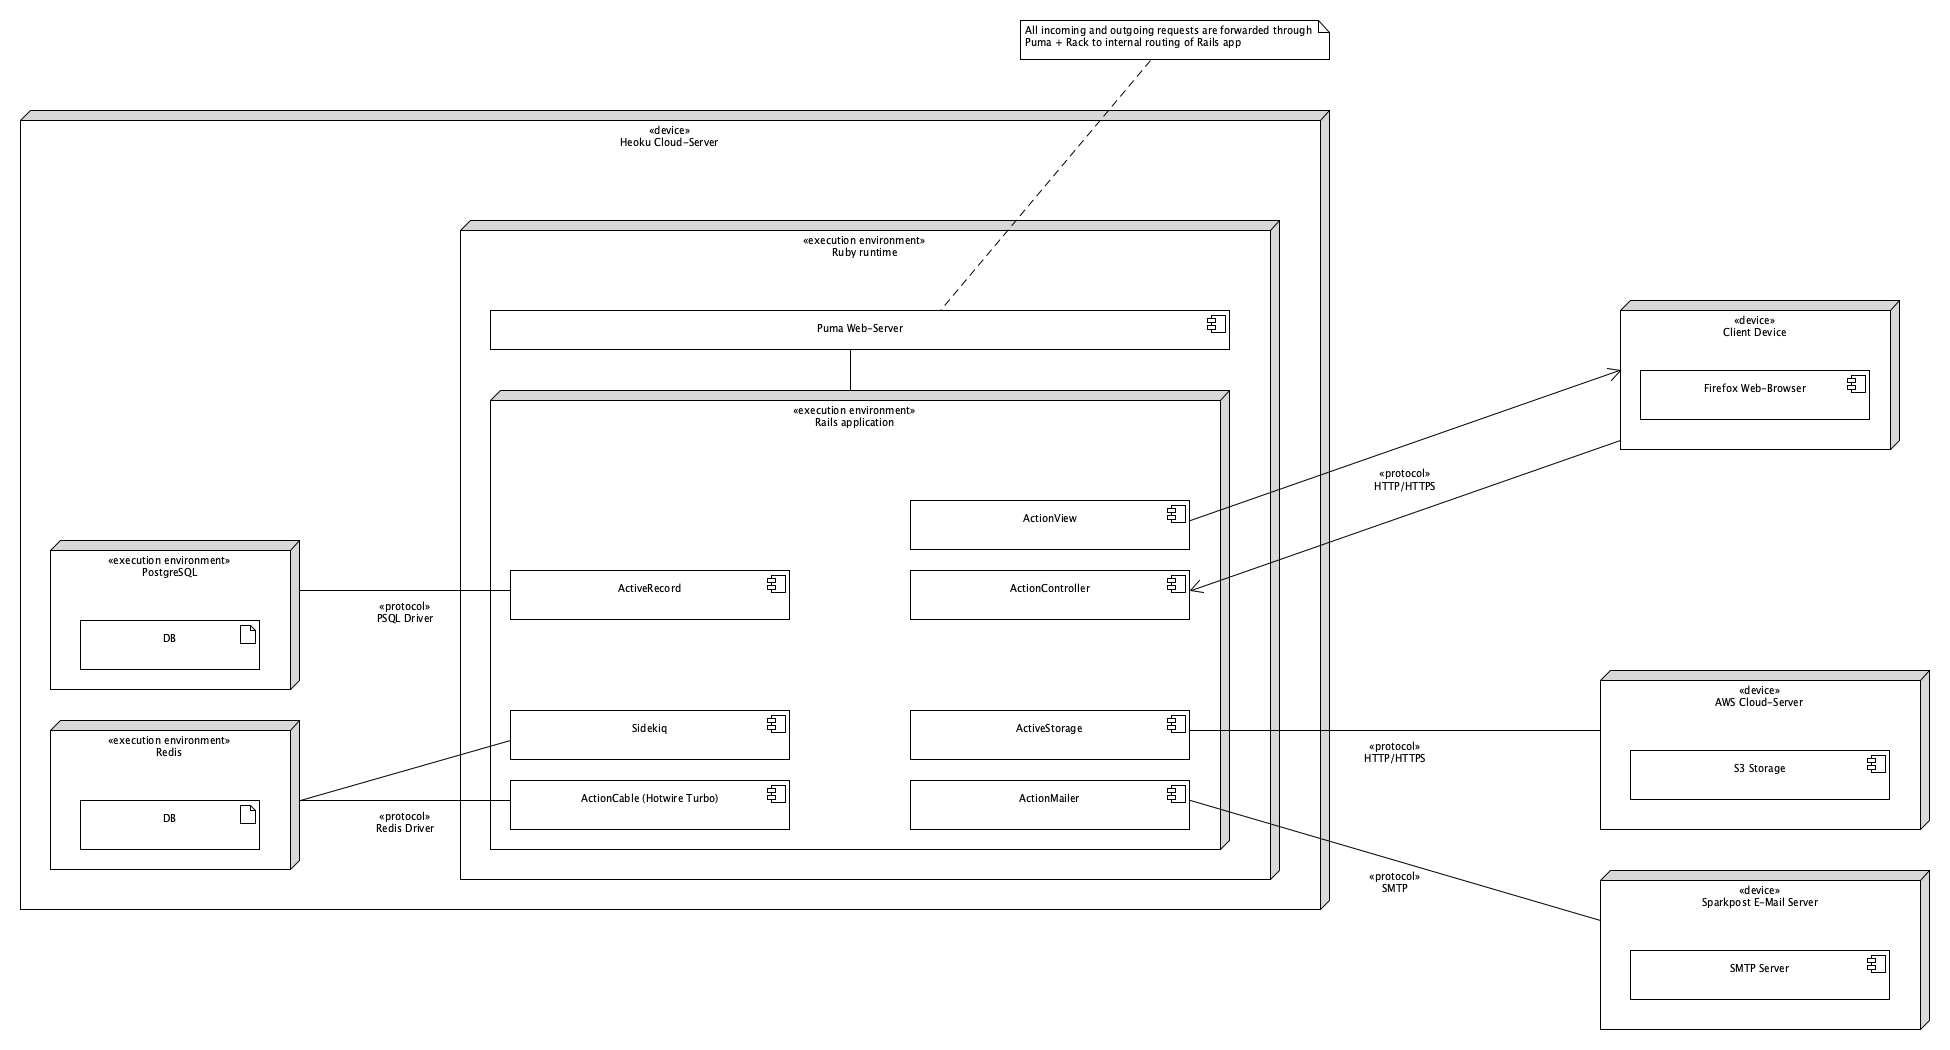
\includegraphics[width=\textwidth]{images/diagrams/deployment.png}
    \caption{\label{fig:deployment}UML Deployment Diagramm}
\end{figure}

\subsection{Systeme und Schnittstellen}

Folgender Abschnitt beschreibt die einzelnen Systeme und Schnittstellen aus der Abbildung \ref{fig:deployment},
wofür sie zuständig sind und wie sie mit dem Kernsystem zusammenhängen und interagieren.

\subsubsection{Heroku}
Heroku ist eine Cloud-Plattform, auf der das Kernsystem gehostet werden soll. Die Plattform bietet eine
Grosszahl von sogenannten Add-Ons und Buildpacks, welche die Skalierung und das Aufsetzten neuer Instanzen unglaublich einfach gestalten.
Dadurch ist man sehr flexibel und kann wichtige Services wie z.B. Datenbanken direkt neben der Haupt-Applikation auf der Selben Plattform hosten.
Neue Versionen werden via git auf den Heroku Server gepusht. Dadurch gestaltet sich auch die Integration der Sempahore CI/CD Pipelines sehr einfach.

\subsubsection{Redis}
Redis ist eine sehr performante in-memory Datenbank, die Daten in Form von Key-Value Paaren speichert.
Die Redis-Instanz wird auf demslben Heroku Cloud-Server in Form eines Add-Ons gehostet. Seit der einführung
von Hotwire in Ruby on Rails 7.0 könnte man es schon fast als ein \enquote{must-have} bezeichnen.
Turbo benötigt eine Redis-Instanz, um temporäre Daten für Websocket Verbindungen zu speichern.

Auch der Job-Scheduler Sidekiq verwendet Redis als eine \enquote{Warteschlange} für Jobs, die in der Zukunft
abgearbeitet werden sollen.

\subsubsection{PostgreSQL}
PostgreSQL - auch \enquote{Postgres} genannt, ist die go-to Datenbank für Ruby on Rails Applikationen,
welche auf Heroku gehostet werden sollen. Eine Instanz der Datenbak wird neben der Rails Application ebenfalls auf einem
Heroku Cloud-Server als Add-On gehostet. Diese interagiert über einen PSQL Datenbanktreiber mit dem ORM gem \emph{ActiveRecord}.
Demnach ist dieses gem dafür züständig, automatisch SQL-Abfragen zu generieren und die daraus resultierenden Records zu Model-Klassen zu mappen und umgekehrt.

\subsubsection{Sparkpost}
Sparkpost ist ein E-Mail Service, den die Renuo AG als Standard in den meisten Softwareprojekten einsetzt.
Auf Heroku können grundsätzlich keine SMTP Server gehostet werden, sodass ein externer Service benötigt wird. Die Sparkpost Instanz
dient hierbei lediglich als Zustellungsserver und kann in diesem Fall keine E-Mails empfangen. Das \emph{ActionMailer} gem baut
E-Mail Templates im Text- oder HTML Format und sendet diese im Anschluss über das SMTP Protokoll an Sparkpost.

\subsubsection{AWS S3}
Neuere Versionen des Ruby on Rails Frameworks beinhalten standardmässig das \emph{ActiveStorage} gem, welches das Hochladen von Dateien auf einen
externen Storage-Service erleichtern soll. Dazu wird in dieser PA der Amazon Simple Storage Service, kurz \enquote{S3} verwendet.
Darauf sollen die Assessment-Lösungen der Bewerber hochgeladen werden.

\subsection{Akteure}

Mit dem System interagieren die folgenden Akteure:

\begin{table}[H]
    \begin{tabular}{|l|l|}
        \hline
        \rowcolor{PrimaryColor!50} Akteur & Beschreibung                                       \\
        \hline
        Bewerber                          & Durchläuft ein Assessment                          \\
        \hline
        Betreuer                          & Koordiniert den Ablauf eines Assessments           \\
        \hline
        Korrektor                         & Korrigiert die Lösungen                            \\
        \hline
        Zeit                              & Erzwingt ein rechtzeitiges Beenden des Assessments \\
        \hline
    \end{tabular}
    \caption{\label{tab:participants} Akteure des Systems}
\end{table}
